
\chapter{My Proposals}
\label{chapt:proposal}


As (section~\ref{setc:ChallengesData} demonstrates, the Megason lab's datasets are hard to proceed. That forces us to find innovative solution for problems that may seem simple at first glance.

This is clear that  the nuclei detection has to be improved.
I started by doing a bibliographic research, to determine the state of the art in the nuclei segmentation/detection domain.
Then, I implemented a new algorithm based on the Laplacian of Gaussian method.
After that, I created an evaluation framework, to compare the results given by this new algorithm, and Kishore's.
We finally proposed a new method taking advantage of the cell membrane information. The following chapter describes its principle.

\section{Principle}

All the papers we have been reading take advantage of the nuclei channel information, but none of them takes advantage of the membrane channel.
This channel provides capital information, especially in the case of stuck nuclei, where most common detection method fail.
Indeed, the membrane can separate the different nuclei.
We propose here a method using the membrane information in an original way.

\section{Theory}


\subsection{preliminaries}


\paragraph{Voronoi diagram}


\paragraph{distance map}


\paragraph{centroïd}


\begin{figure}[h]
\begin{center}
\leavevmode
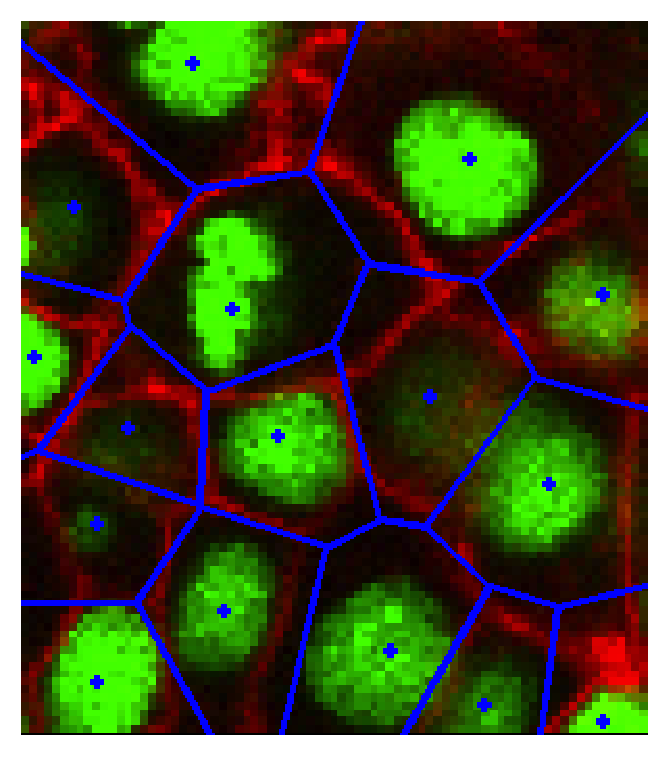
\includegraphics[width=0.5\textwidth]{pictures/voronoiExample2D}
\end{center}
\caption{Voronoi diagram (blue) centred in each cell nuclei (green), with the membrane (red)}
\label{fig:voronoiExample2D}
\end{figure}
Several article make use of Voronoi diagrams to delimiter the zone where one nuclei is present.
But the membrane is also around each nuclei. So the membrane channel provides us with information about nuclei positions.
We can see figure~\ref{fig:voronoiExample2D}, that the membrane can be approximated by a Voronoi diagram centred in each nucleus.
From this, we can use the membrane channel and consider it as a Voronoi tessellation, and from this, find the Delauney triangulation.
The triangulation's intersections would be the centres of the cells. And nuclei are most of times located next to the center of the cell.

\paragraph*{}



The Voronoi cells are constituted by all the points closer to the center of the cell than any other center. Thus, if we draw a distance map from the Voronoi cells, the local maximas of this distance map are the centres.
We want to take advantage of this principle by drawing a distance map on the membrane channel. For the localizing the local maximas, there is no need for a complete membrane information, as illustrated figure~\ref{fig:incompleteMembraneSynthetic}.
\begin{figure}[h]
  \centering
\subfloat[Synthetic Voronoi cell]{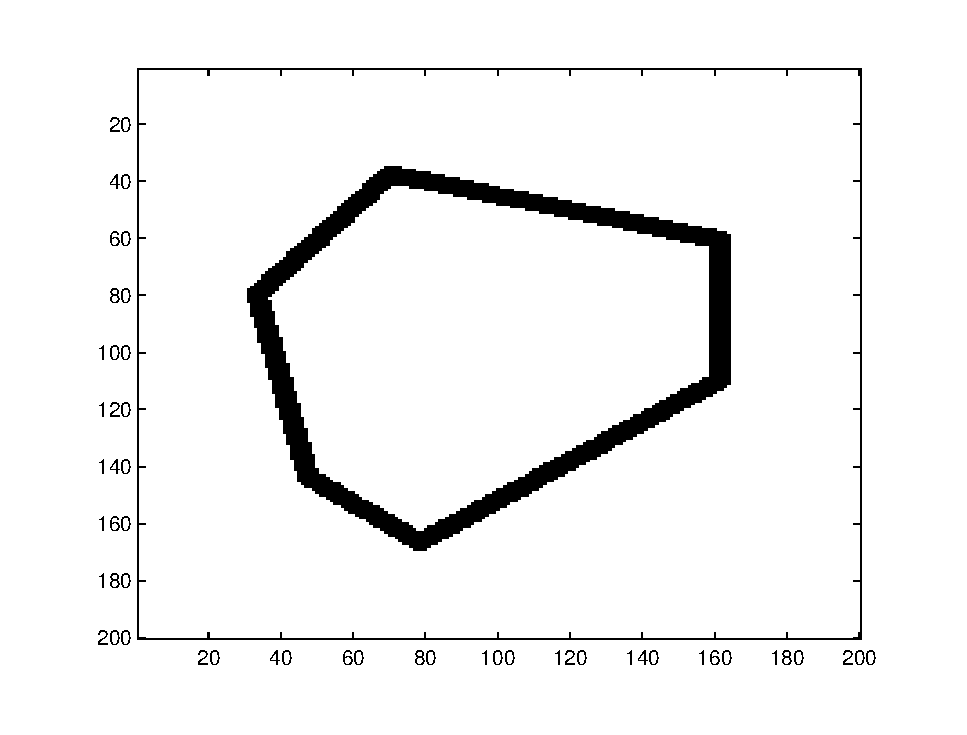
\includegraphics[width=0.49\textwidth]{pictures/membraneCellFull}\label{fig:membraneCellFull}}
\subfloat[Degraded synthetic Voronoi cell]{\includegraphics[width=0.49\textwidth]{pictures/membraneCellIncomplete}\label{fig:membraneCellIncomplete}}\\
\subfloat[Distance map computed from the synthetic Voronoi cell (figure~\ref{fig:membraneCellFull}). We clearly see a local maxima in the center of the cell.]{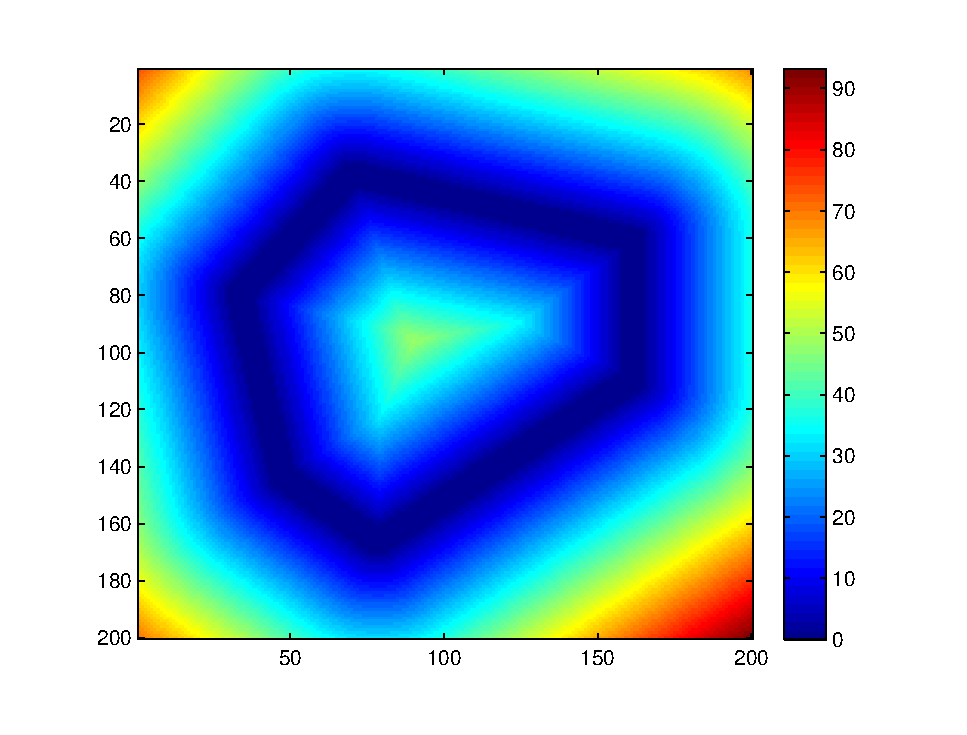
\includegraphics[width=0.49\textwidth]{pictures/membraneCellFullDistance}\label{fig:membraneCellFullDistance}}
\subfloat[Distance map computed from the degraded synthetic Voronoi cell (figure~\ref{fig:membraneCellIncomplete}). The local maxima is still in the center of the cell.]{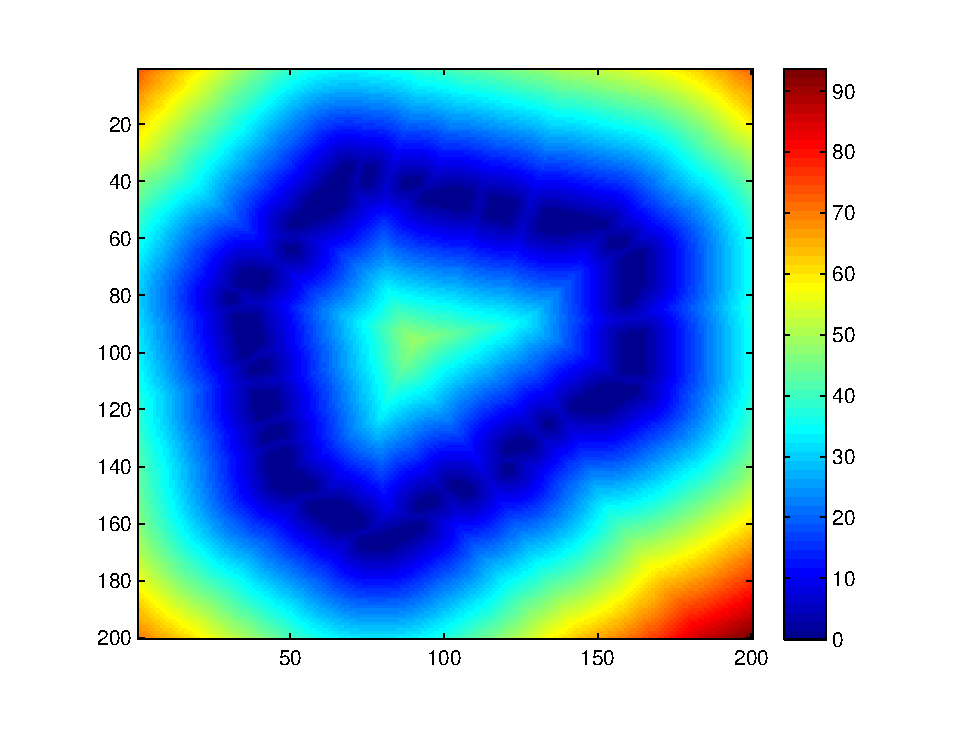
\includegraphics[width=0.49\textwidth]{pictures/membraneCellIncompleteDistance}\label{fig:membraneCellIncompleteDistance}}
\caption{Center of Voronoi cell stay unchanged under important degradation of the cell borders.}
  \label{fig:incompleteMembraneSynthetic}
\end{figure}



\subsection{Description}
We have seen that we can work on degraded membrane data to find an approximate position of cell nuclei.
We will now describe the innovative membrane reconstruction step that Kishore Mosaliganti developed and that we use in this algorithm.


This reconstruction is based on a diffusion filter pre-processing. The diffusion filter locates planar structures in the 3D data, and diffuses intensities along these plans.
We get a good first approximation of the membrane with this method, but many holes are still present.
In order to fill some of them, and reconnect the membrane, Kishore M.~{\etal} use a technique known as tensor voting.
This reconnect disconnected points, by finding privileged local directions.

The reconstruction of the membrane is illustrated figure~\TODO{reconstruction illustrations}.

This is the membrane information that we will use for finding the cell centres.







\subsubsection{Algorithm pipeline}

It is clear that for most image processing problems, a series of transformation is needed in order to be able to work with the data.
Inspired by the described articles, I designed an image processing pipeline adapted to our data.
I describe here the image processing pipeline for the new algorithm, and the improvements of the existing nuclei segmentation pipeline
\begin{description}
  \item[Denoising: ] We first process the membrane and the nuclei channel with a median filter. The median filter's structuring element is a disk of radius
  \TODO{radius of the median finally?}.
  We don't process directly the very low third dimension, as we may lose some relevant data,
  thus, the filter's structuring elements is two dimensional and applied to each "slice" (xy plan).
%
%
  \item[Images Resampling: ] As in \cite{li20073}, our images are anisotropic : they are very high resolution in xy, and very low resolution in z, as shown by the
  table~\ref{tab:DataSizes}, and the figure~\TODO{reference to the anisotropy figure in data analysis}.
  We don't need this much information in xy, as algorithms are computationally expensive, and we want to keep a reasonable processing time.
  But, we need a higher resolution in z.
  For that purpose, we resample our images, using a BSpline interpolation of order 5.
  This technique provides us with an isotropic dataset of spacing 0.4um, that can easily be
  processed by the other filters. The interpolation, in the z direction, partially reconstructs the membrane.
%
%
  \item[Nuclei binary mask: ] We threshold the nuclei image to keep a rough binary mask in which the nuclei are present.
  The thresholds are chosen after an analysis of the histogram of the nuclei images.
%  
  \TODO{image of the binary mask}
%
%  
  \item[Distance map creation: ] We then process the resampled and denoised membrane channel with Kishore's membrane reconstruction filter.
  The resultant membrane is thresholded to get a binary image from which we compute a distance map
  using the algorithm proposed by Maurer Jr {\etal}~\cite{maurer2003linear}.
  The threshold values are empirically determined.
%  
  \TODO{display distance map}
%
%
  \item[Local maxima extraction: ] Then, we dilate the distance map, This method is useful for local maxima extraction:
  it merges local maximas to keep the highest one, in a region defined by the structuring element's radius.
  After dilating the distance map according to , we locate local maximas with the flooding algorithm described in\cite{beare2005finding}.
  We only select local maximas that can possibly be located in the center of a cell, thus eliminating low values and high values corresponding respectively to holes in the membrane channel, and structures of the fish without cell.
%  
  \TODO{display dilated distance map}
%
%
\end{description}


\subsection{Evaluation}

It is important to note that often times, Biologists just want to count and localize objects in an image, without segmenting them.
That's why, in order to only evaluate the nuclei detection step, excluding the watershed segmentation, I created an evaluation framework providing necessary informations such as:
 out of nuclei detection (false positive), over detection of a nuclei (false positive), non detection of a nuclei (false negative) and correct detection of a nuclei.

I also created some tools for comparison of 3D datasets (based on {\gofigure}), and for simultaneous visualisation of point cloud and ray casted 3D dataset.

We will evaluate three algorithms in this section:
the algorithm that was used when I arrived in the Megason Lab (see section~\ref{sect:megasonExisting}),
the variant of the Laplacian of Gaussian presented in \cite{al2009improved} (see section~\ref{sect:farsight}),
and our proposed algorithm (see section~\ref{sect:proposal}).


\subsubsection{evaluation on synthetic data}

The generated synthetic data simulate the point-spread function of the microscope, on blobs, representing nuclei, and on Voronoi tessellations, representing membranes.
The data has a low resolution in z.
It is possible to have a variable noise level, and we will use these data to experience the robustness of the evaluated algorithms.

\begin{figure}[htb]
\begin{center}
\begin{tabular}{|c|c|c|c|c|}
\hline Noise level & Nuclei count & Correctly detected & Over-detected & Not-detected \\ 
%\hline x (space) & 1024 & 0.24 um & \\ 
\hline
\end{tabular} 
\end{center}
\caption{Evaluation of 3 algorithms on different synthetic datasets.}
\label{tab:DataSizes}
\end{figure}

\subsubsection{evaluation a segmented dataset}

We currently have one segmented dataset in the Megason Lab. The dataset is a part of an ear imaged 2 year ago. It is populated with a lot of noise. The region of interrest of the dataset (which has been manually segmented), contains \TODO{hox many cells in synthetic dataset ?} nuclei.
We ran the algorithms on the whole dataset, and masked the detection results with the region of interest.

\begin{figure}[htb]
\begin{center}
\begin{tabular}{|c|c|c|c|}
\hline Nuclei count & Correctly detected & Over-detected & Not-detected \\ 
%\hline x (space) & 1024 & 0.24 um & \\ 
%\hline y (space) & 1024 & 0.24 um \\ 
\hline
\end{tabular} 
\end{center}
\caption{Evaluation of 3 algorithms on a manually segmented dataset.}
\label{tab:DataSizes}
\end{figure}

\subsubsection{results}

\TODO{}
We found that THIS algorithm is more accurate, that THIS one is more robust, that THIS one is faster, that OURS is ...

\subsection{conclusion \& future}


We can improve the proposed algorithm, by automating the choice of the thresholds based on histograms.
We could also use non linear resampling methods, for improving the resolution among z.

We also implemented a Kdtree for grouping the local maximas, instead of using a dilation of the distance map,
such implementation would require a time evaluation, as the distribution of local maximas in space affects the effectiveness of the Kdtree requests.

We could combine the use of algorithms : the membrane based one in regions where nuclei are clumped, and the contour based ones (Kishore's or the improved Multiscale Laplacian of Gaussian) in region where nuclei are isolated.
The detection of such regions can be done by analysing the size of the connected components of the binarized nuclei image:
clumped nuclei correspond to large connected components.

\section*{Conclusion}


%A Context of the internship
%1- Biological Context / Goals
%2- Image Processing Challenges
%3- Data presentation
%4- The problem: you are going to address " ??? "
%
%B- Cell nuclei detection
%Intro
%1- State of the art
%2- What's wrong with existing method
%3- Your proposal
%4- Results
%    1- Synthetic data
%    2- Real data
%    3- Comparison of your method vs the other one. Validation? What is the benefit?
%5- Partial conclusion.
%    1- What is new?
%    2- Did you improve existing methods? in which way?
%        if not, why?
%    3- Future work.
%
%C- Membrane segmentation
%Intro
%1- State of the art
%2- What's wrong with existing method, if any?
%3- Your proposal (using a watershed starting from seeds)
%4- Results
%    1- Synthetic data
%    2- Real data
%    3- Comparison of your method vs the other one. Validation? What is the benefit?
%5- Partial conclusion.
%    1- What is new?
%    2- Did you improve existing methods? in which way?
%        if not, why?
%    3- Future work. 





%
%
%\subsection{Laplacian of Gaussian implementation}
%\label{sect:MLOG}
%\subsubsection{Strategy}
%
%\TODO{mettre dans les commentaires de farsight, improvements}
%
%The idea was to reimplement only the part of the algorithm of \cite{al2009improved} concerning the cell nuclei detection.
%The goal being to improve our initialization of the watershed algorithm. I was able to work with Raghav K. Padmanabhan, from the Roysam lab (who develops FTK),
%during the NA-MIC\footnote{The National Alliance for Medical Image Computing (NA-MIC) is a multi-institutional, interdisciplinary team of computer scientists,
%software engineers, and medical investigators who develop computational tools for the analysis and visualization of medical image data.} summer project week, in MIT.
%We tried to apply the FTK nuclei detection technique to 3D datasets, and to extract the Scale-constrained Laplacian of Gaussian implementation from the source code.
%
%A visual comparison of the binarization proceed by Kishore's algorithm and by the Farsight ToolKit led to the conclusion that Kishore's binarization
%was proceeding longer, but providing smoother results, which are important for the distance map step. That's the reason why, for the comparison of both algorithm,
%I reimplemented the Scale Constrained Laplacian of Gaussian and integrated it to Kishore's processing pipeline.
%
%
%\subsubsection{Implementation}
%After reading and understanding the article, I checked out the code from the Farsight Toolkit. The code has been developed two years ago and is not maintained any more.
%There was few documentation and comments, and the use of global variables made it hard to understand.
%I decided to start from scratch and reimplement the algorithm.
%
%The datasets are huge in the Megason Lab, and in order to process them, Kishore develops all his algorithms in \C++ with the Insight ToolKit (ITK) library.
%It was necessary that I develop the multi-scale Laplacian of Gaussian and create the whole evaluation framework with this language.
%
%
%\subsubsection{Testing}
%
%Prior to evaluating the algorithm, it was necessary to test it on some well known data.
%Indeed, The ITK implementation of the Multiscale Laplacian of Gaussian has a documentation and implementation problem:
% the code and the documentation are contradictory about the normalisation across scales.
%I tested the algorithm on a known function to verify its functioning.
%
%The test image was a 2D Gaussian of unit energy (integration across space equals one),
% and of different standard deviation. If the normalisation across scales is working,
%  the result of the Laplacian of Gaussian should be the same if computed across enough scales.
%\TODO{find the test for multiscale log on gaussian.}
%We proved the filter to be effectively working and detecting blobs of different scales without a loss in intensity as scale increases.
%\TODO{provide test for several scales}
%



%A "Plan of the internship"
%1 Goal (segment cells & membrane)
%2 Data presentation
%3 Where are we ? (membrane seg~0 cell seg needs lots of improvements)
%priority seeding imposed
%
%B Cell nuclei detection
% Intro
%bad seeding as of now, new ago, need for evaluation
%
%2 Biblio
%biblio on seeding evaluation
%
%3 Implementation
%implemantation … hard very hard (go through other's code forgotten already...)
%
%4 proposing
%new ago proposition new approach (based on membrane information)
%
%5 testing
%result of evaluation
%
%6 difficulties and future
%implementation big datasets 3D …
%future : merge results ? first : bad results everywhere : no more info for merging seedings...
%other ago based on wavelets? (as an opening)
%
%C Membrane segmentation
%  intro
%challenging need good cell detection...(but none present yet)
%1 biblio
%2 implementation (only 2D)
%3 result (only 2D)
%long very long but implementation can be greatly improved
%4 future
%not based on cell detection (start growing on the membrane)



%
%
%
%
%
%\section{Segmentation de la membrane cellulaire par ensembles de niveaux}
%
%Le but initial du PFE etait la segmentation de la membrane cellulaire. il s'agit d'une fine membrane séparant les multiples cellules. Elle s'étend sur tout le spécimen à analyser. Il s'agit donc d'un volume important et complexe.
%
%\subsection{Étude du problème}
%
%J'ai tout d'abord cherché à comprendre le problème posé : sur quelles données allaient se baser la détection, existe-t'il des solutions pour segmenter ce genre de données.
%
%\subsubsection{Les données}
%Les images sont acquises a travers un système optique. L'excitation par un laser entraine la fluorescence de certaines parties de la cellule, marquées par une molécule émettant de la lumière dans un spectre dépendant du marqueur utilisé.
%
%Le système a donc une réponse impulsionelle bien visible dans les données. Un point correspond grossièrement a une gaussienne étalée dans les trois dimensions de l'espace, et plus particulièrement selon l'axe perpendiculaire au plan de focalisation.
%
%Il existe aussi un bruit dû au dispositif électronique d'acquisition. De plus, la fluorescence n'étant pas répartie de manière homogène, il existe des "trous" et de la saturation dans les données.
%\TODO{inserer des images illustrant les problemes}
%
%
%J'ai choisi de me focaliser sur trois difficultés afin de trouver des solutions :
%\begin{description}
%  \item [problème du bruit] : quel filtrage appliquer aux images, afin de les débruiter.
%  \item [problème de l'absence de données] : comment introduire des à priori de forme de la membrane
%  pour palier à l'absence d'information ?
%  \item [problème de la non homogénéité des intensités]  : comment segmenter un objet
%  qui n'occupe pas les mêmes intensités selon sa position dans l'espace.
%\end{description}
%
%
%\subsection{Débruitage des données}
%Le bruit présent sur les images n'est pas gaussien. Il n'est pas répartis de la même manière dans toute l'image non plus. Je me suis donc focalisé sur des techniques de débruitage telles que le filtre médian, et plus généralement des filtres morphologiques.
%
%Le filtre médian donne de bons résultats, pour un temps de calcul inférieur aux filtres morphologiques (reconstruction par dilatation/erosion)
%
%\subsection{Segmentation de la membrane}
%
%\subsubsection{Utilisation de la théorie des ensembles de niveaux}
%
%L'outil choisi pour segmenter la paroi cellulaire, est base sur les ensembles de niveaux (levels-sets). Cette théorie consiste en l'évolution d'un front. Cette évolution est représentée par une fonction implicite qui évolue itérativement. Le front (bords de la zone segmentée) est souvent représenté par le niveau zéro de cette fonction implicite.
%Les Level sets, au travers de leur critère d'évolution, permettent d'avoir une grande flexibilité quand aux mesures a considerer lors de l'evolution du front. Cette évolution est représentée par un critère d'énergie, le problème de segmentation par level set est donc un problème d'optimisation.
%
%\subsection{des idees}
%
%
%
%
%
%
%idee de la mediane
%idee morphologie
%idee localisation
%\subsection{resultats}
%idee mediane
%idee morphologie
%idee localisation
%\subsection{travail futur}
%rapidite
%
%
%
%\section{Detection et localisation des cellules}
%
%Nous basons nos méthodes de segmentation sur une initialisation au centre des cellules. Nous avons donc besoin de détecter un maximum de cellules afin de trouver un point a l'intérieur de ces dernières. Des methodes ont ete proposees, cependant, chacune est adaptee a un type d'image particulier.
%Cels algorithmes de détection sont aussi souvent appelles algorithmes de "seeding" car ils permettent d'obtenir des points a partir desquels une segmentation peut etre initialisee, afin de delimiter les bordures des noyaux, ou les membranes cellulaires.
%
%\subsection{demarche}
%
%Nous avons developpe une methode combinant l'information provenant des noyaux et de la membrane des cellules. Cette methode doit etre evaluee, donc comparee a d'autres methodes existantes. Ce processus d'evaluation nous permettra aussi de trouver les points forts et les points faibles des algorithmes. Nous pourrons ainsi eventuellement utiliser des techniques de fusion d'information pour combiner les resultats de differents algorithmes.
%La creation d'un "framework" d'evaluation passe donc par plusieurs etapes : l'implementation des algorithmes existants, afin de les tester sur des images synthetiques puis reelles, la creation de criteres d'evaluation appropories, et l'observation des resultats. Nous avons aussi initié un travail afin de proposer une nouvelle methode de detection de cellules basee sur la decomposition en ondelettes.
%
%
%\subsection {description des algorithmes evalues}
%
%
%
%\subsubsection{chaine de traitement de l'image}
%
%partie commune
%Nous nous focalisons sur une classe d'algorithmes traitant l'information issue de l'image des noyaux cellulaires, apres une detection des zones d'interet (binarisation de l'image). Ces algorithmes fonctionnent aussi souvent avec une extraction de maxima locaux en dernier traitement.
%Nous choisissons d'utiliser la même binarisation, et la meme methode d'extraction de maximas locaux pour les deux algorithmes afin de focaliser l'etude sur la technique de detection des centres des noyaux.
%
%\subsubsection{description des algorithmes}
%\paragraph{le Laplacien de la Gaussienne ameliore}
%Nous avons decide d'implementer l'algorithme presente dans \cite{al2009improved}. La methode utilisee est celle du Laplacien de la Gaussienne (LoG). Une methode eprouveee qui s'est montree tres robuste dans d'autres applications telles la detection de points de reperes pour le recallage photographique.
%
%
%
%\paragraph{Kishore}
%
%\TODO{Ask Kishore more infos}
%
%
%\subsection {evaluation}
%%\begin{tabular}{|c|c|c|c|c|}
%%\hline  & Matching & UnMatching & Missed & Accuracy \\ 
%%\hline A1 & 10 & 3 & 1 & 71% \\ 
%%\hline A2 & 9 & 2 & 3 & 64% \\ 
%%\hline 
%%\end{tabular} 
%
%
%
%\subsection {conclusion}
%
%
%\subsection {proposition}
%
%
%
%\subsection {planning}
%
%
%\subsection{resultats}
%
%\subsection{proposition}
%
%
%
%
